\documentclass[a4paper,twoside]{book}
\usepackage{rutitlepage}
\usepackage{url}
\usepackage{geometry}
\usepackage[english]{babel}
\usepackage{lipsum,etoolbox}
\usepackage[nodayofweek]{datetime}
\usepackage[toc,acronym,shortcuts]{glossaries}
\usepackage{listings}
\usepackage{float} % Pictures
\usepackage[backend=biber,style=numeric,maxbibnames=5]{biblatex}
\usepackage{subcaption} %subfigure
\usepackage[export]{adjustbox} % subfigure
\usepackage{graphicx} %subfigure
\usepackage{lmodern}
\usepackage{hyperref} %Clickable links

% -------- Resources --------
\addbibresource{thesis/thesis.bib}

\usepackage{listings}
\usepackage{stmaryrd}

% color definitions
% the following colors are appealing for background of code segments
%CornflowerBlue    heldere blauwe kleur
%CadetBlue         sobere blauwe kleur
%Periwinkle        blauw die neigt naar paars, nogal donker
%Thistle           wat valere kleur, minder nadrukkelijk aanwezig
%YellowOrange      erg nadrukkelijke kleur
\newcommand{\ExampleCodeBackgroundColor}{\color{White}}
\newcommand{\ExampleCodeFrameColor}{\color{black}}
\newcommand{\CleanDocFrameColor}{\color{black}}


\lstdefinelanguage{Clean}{%
	alsoletter={ABCDEFGHIJKLMNOPQRSTUVWXYZabcdefghijklmnopqrstuvwxyz_`1234567890},
	alsoletter={~!@\#$\%^\&*-+=?<>:|\\.\\{\\}},
	morekeywords={generic,implementation,definition,dynamic,module,import,from,where,in,of,case,let,infix,infixr,infixl,class,instance,with,if,derive,code},
	sensitive=true,
	escapeinside={[+}{+]},
	morecomment=[l]{//},
	morecomment=[n]{/*}{*/},
	morestring=[b]",
	morestring=[s]{['}{']},
	basewidth=0.43em,
	columns=[c]fixed,
	texcl=true,
	literate=%
		% Basic Clean constructs
		%{\\}{{$\lambda\:$}}1
		%{::}{{$:\!\!\!:$}}1
		%{:.}{{$:\!.$}}1
		{...}{{.\!.\!.}}2
		%{++}{{$+\!+$}}2
		%{+++}{{$+\!\!\!+\!\!\!+$}}2
		%{==.}{{==\!.}}2
		%{=.}{{=\!.}}1
		%{>=}{{$\geq\:$}}1
		%{<=}{{$\leq\:$}}1
		%{||-}{{$\mid\mid\!$-}}2
		%{-||}{{-$\!\mid\mid$}}2
		%{-||-}{{-$\!\mid\mid\!$-}}2
		%{-&&-}{{-$\!\&\!\&\!$-}}4
		{not}{{$\neg$}}1
		{->}{{$\shortrightarrow$}}1
		{<<@}{{$\ll\!\!@$}}2
		%{>>=}{{$\gg\!\!=$}}2
		%{>>*}{{$\gg\!\!\!\!^*$}}2
		%{>>|}{{$\gg\!\mid$}}2
		{A.}{{$\forall\;\,$}}1
		%{E.}{{$\exists\;\,$}}1
}


\lstdefinestyle{cleanStyleInline} {
    breakatwhitespace,
    breaklines
}

\newcommand{\CleanInline}[1]{\lstinline[language=Clean,style=cleanStyleInline];#1;}
\newcommand{\Cl}[1]{\CleanInline{#1}}
\newcommand{\CI}[1]{\lstinline[language=Clean,basicstyle=\ttfamily\fontseries{l}\normalsize]|#1|}

\lstdefinestyle{numbers}{numbers=right, stepnumber=1, numberstyle=\tiny, numbersep=-5pt}

% environments for documentary code segments
\lstnewenvironment{CleanDoc}{\lstset{language=Clean}}{}
\lstnewenvironment{CleanDocN}{\lstset{language=Clean,style=numbers}}{}
\lstnewenvironment{CleanDocB}{\lstset{language=Clean,frame=single,rulecolor=\CleanDocFrameColor}}{}
\lstnewenvironment{CleanDocNB}{\lstset{language=Clean,style=numbers,frame=single,rulecolor=\CleanDocFrameColor}}{}

% environments for example code segments
\lstnewenvironment{CleanEx}{\lstset{language=Clean,frame=single}}{}
\lstnewenvironment{CleanExN}{\lstset{language=Clean,style=numbers,frame=single,rulecolor=\ExampleCodeFrameColor,backgroundcolor=\ExampleCodeBackgroundColor}}{}

\lstset{
    language=Clean,
    showstringspaces=false,
    basicstyle=\ttfamily,
    frame=leftline}

\makeglossaries
\newacronym{adt}{ADT}{Algebraic Data Type}

\newacronym{dsl}{DSL}{Domain Specific Language}

\newacronym{edsl}{E\acs{dsl}}{Embedded \acl{dsl}}

\newacronym{gadt}{GADT}{Generalized Algebraic Data Type}

\newacronym{gpl}{GPL}{General Purpose Language}

\newacronym{html}{HTML}{Hypertext Markup Language}

\newacronym{iot}{IoT}{Internet of Things}

\newacronym{sds}{SDS}{Shared Data Source}

\newacronym{top}{TOP}{Task Oriented Programming}

\newacronym{vhdl}{VHDL}{\acs{vhsic} Hardware Description Language}

\newacronym{vhsic}{VHSIC}{Very High Speed Integrated Circuit}

\newacronym{led}{LED}{Light-Emitting Diode}

\newacronym{midi}{MIDI}{Musical Instrument Digital Interface}

\newacronym{eeprom}{EEPROM}{Electrically Erasable Programmable Read-Only Memory}

\newacronym{ghc}{GHC}{Glasgow Haskell Compiler}

\newacronym{uav}{UAV}{Unmanned Air Vehicles}

\newacronym{frp}{FRP}{Functional Reactive Programming}

\newacronym{ota}{OTA}{Over-the-Air}

\newacronym{ide}{IDE}{Integrated Development Environment}

\newacronym{lan}{LAN}{Local Area Network}

\newacronym{ui}{UI}{User Interface}

\newacronym{lcd}{LCD}{Liquid Crystal Display}

\newacronym{posix}{POSIX}{Portable Operating System Interface}

\newacronym{arm}{ARM}{Advanced RISC Machine}

\newacronym{risc}{RISC}{Reduced Instruction Set Computer}

\newacronym{tcp}{TCP}{Transmission Control Protocol}

\newacronym{pir}{PIR}{Passive Infrared Sensor}

\newacronym{usb}{USB}{Universal Serial Bus}

\newacronym{ip}{IP}{Internet Protocol}

\newacronym{spp}{SPP}{Serial Port Protocol}
% ----------------------------

% --------- Commands ---------
\newcommand{\projecttitle}{Developing Real Life, Task Oriented Applications for the Internet of Things}
\newcommand{\rinus}{prof.~dr.~dr.h.c.~ir.~M.J.~Plasmeijer }
\newcommand{\pieter}{dr.~P.W.M. Koopman}
\newcommand{\mart}{M. Lubbers MSc.}
\date{\today}
\author{Matheus Amazonas Cabral de Andrade}
\urlstyle{tt}
% ----------------------------


\begin{document}
\frontmatter{}

% -------- Title Page --------
\maketitleru[
    layout=seventeen,
    title=Master's Thesis,
    subtitle=\projecttitle,
    others={{Supervisor:}{\rinus},{Daily Supervisor:}{\mart},{Second Reader:}{\pieter}}]
\clearpage
% ----------------------------

% --------- Abstract ---------
\chapter*{\centering Abstract}
    \addcontentsline{toc}{chapter}{Abstract}
    The \acl{iot} is becoming ubiquitous. A growing number of objects are being equipped with devices that interact with its environment and exchange data via the Internet. Such devices are not powerful enough to run \gls{iTasks} (an implementation of the \acl{top} paradigm written in \gls{clean}) applications. The \gls{mTask} \acl{edsl} was created with one goal in mind: to bring \acl{iot} devices and the \acl{top} paradigm together. But so far, only trivial applications were developed using \gls{mTask}. This thesis assesses whether \gls{mTask} can be used to develop real-life applications. \gls{autohouse}, 
the home automation application developed during the research, guided improvements in the \gls{mTask} development environment and unearthed problems yet to be resolved.
% ----------------------------
    
% ----- Acknowledgements -----
\chapter*{\centering Acknowledgements}
    \addcontentsline{toc}{chapter}{Acknowledgements}
    I would like to thank everyone that helped me directly or indirectly in this adventure. Rinus and Mart for the supervision, weekly meetings, patience, advice and continuous feedback. Pieter for the help during the thesis and the feedback provided on this report. My friends around the globe that somehow overcame the distance and pushed me towards my goals. My Nijmegen friends for the daily advice, encouragement and occasional de-stressing parties. Last but not least, I would like to thank my family for the continuous support during these two last years. There is no doubt that I only made this far because of you. I love you. Specially, I would like to thank my parents for always trusting me and pointing me in the right direction. 


% ----------------------------

% ---- Table of contents -----
\tableofcontents
\clearpage
% ----------------------------

\mainmatter{}

% -------- Chapters ----------
\chapter{Introduction}
    \section{Introduction}
The \ac{iot} consists of a network of "things" (devices, computers, people, systems, etc) where its components interact with each other via the Internet. These components can exchange data, monitor and manage each other. \ac{iot} is a global, growing phenomenon. According to Gartner~\cite{iot_numbers}, there were 3.96 billion connected "things" in 2016 and by 2020, 12.863 billion devices are expected to be connected to the Internet. \ac{iot} is being used in a myriad of applications including house automation, fitness tracking, health care, warehouse monitoring, agriculture and industry manufacturing. \ac{iot} devices can be dedicated servers, personal computers, tablets, smartphones, smartwatches or compact devices operated by microcontrollers. Microcontrollers are small, cheap computers with limited resources and low power consumption commonly used to interface with the real world. They often gather data from sensors (movement, light, temperature, etc), act on actuators (motors, LEDs, swtiches, etc) and communicate with other devices.


%often connected to sensors (movement, light, temperature, etc) and actuators (motors, LEDs, switches, etc). They are commonly used to interface with the real world on a 

% Structure: 
%   IoT ---
%   TOP and iTasks
% mTask


\section{Research Question}
\section{Report Structure}

This report is structured as follows. Chapter \ref{chap:intro} contains the introduction, research question and report structure. Chapter \ref{chap:edsl} quickly introduces \acp{dsl} and presents different strategies to build \acp{edsl}. Chapter \ref{chap:top} introduces the concept of \ac{top} and the iTasks library. Chapter \ref{chap:mtask} presents the mTask \ac{edsl}, which was the research focus. Chapter \ref{chap:application} describes the real-life application developed during research. Chapter \ref{chap:dev} details the development process. Chapter \ref{chap:conclusion} concludes presenting insight about the development process, answering the research question and proposing future research. Chapter \ref{chap:related} lists related work.

The source code for the real-life application developed during research can be accessed at \url{https://github.com/matheusamazonas/autohouse}.

The source code of the modified version of mTask used during research can be accessed at \url{https://gitlab.science.ru.nl/mlubbers/mTask/tree/peripherals}.

The source code of this report can be accessed at \url{https://github.com/matheusamazonas/masterthesis}.

%The source code of the library to interface with the DHT22 temperature and humidity sensor can be accessed at \url{https://github.com/matheusamazonas/DHTino}.

%The source code of the library to interface with the HC-SR04 ultrasonic sensor can be accessed at \url{https://github.com/matheusamazonas/Ultrino}.

\chapter{Embedded Domain Specific Languages}
    A \ac{gpl} is a computer language intended to be used in a wide range of domains. An example is the C++ programming language, which can be used in domains that vary from video games to web servers and systems programming. In contrast, a \acf{dsl} is a computer language that was designed to be used in a particular domain. Game Maker Language, \acs{html}, LaTeX and \acs{vhdl} are examples of \acp{dsl}. These languages, when compared to \acp{gpl}, offer a higher level of abstraction from their target domain.

A \ac{dsl} can be implemented using two different strategies: standalone and embedded. Each strategy has its advantages and disadvantages. In the former strategy, the language is built from the ground up, which consists of developing either a compiler or an interpreter. This strategy provides the language designer with a lot design freedom, but requires a cumbersome amount of work. In the latter strategy, the proposed \ac{dsl} is embedded in another language. Therefore, the \ac{dsl} inherits functionality from its host language. This inheritance often is desirable (e.g., a type checker) but sometimes might be undesirable (e.g., type coercion). This strategy frees its designer of building a new compiler.

The semantics of a \acf{edsl} are given by its views (also called backends). Common views are evaluation, pretty printing, compilation, optimization and verification. There are two main techniques for building an \ac{edsl}: deep and shallow embedding.

\section{Deep Embedding}

Building a deeply \ac{edsl} consists of representing language constructs as \acp{adt} in the host language. Views are functions that take the \ac{adt} as input and return another \ac{adt} that represents its semantics. An example of a simple deeply \ac{edsl} and its views (pretty printing and evaluation) can be seen on Listing \ref{deep1}.


\begin{lstlisting}[caption=A simple deeply \ac{edsl} and its views,captionpos=b,label=deep1]
:: MyDSL = I Int
    | B Bool
    | Add MyDSL MyDSL
    | Sub MyDSL MyDSL
    | And MyDSL MyDSL
    | Or MyDSL MyDSL
    | Var String
    
prettyPrint :: MyDSL -> [String]
eval :: MyDSL -> Int
\end{lstlisting}

The biggest advantage of deep embedding is that adding a view to the \ac{dsl} is easy: simply create a function that transforms the \ac{adt}. One disadvantage is that extending the \ac{dsl} might require a lot of work, since new code has to be created for every new construct in all the views. Another disadvantage is its lack of static type safety. As seen on Listing \ref{deep1}, \texttt{MyDSL} allows operations on mixed data types, as addition on booleans and disjunction on integers. In addition, variables are checked at runtime instead of compile time.

\acp{gadt} can be used to accomplish static type safety in deeply \acp{edsl}, but they do not enable compile time variable checks~\cite{gadts}. 

\section{Shallow Embedding}
Building a shallowly \ac{edsl} consists of representing the language constructs directly as its semantics. An example of a simple shallowly \ac{edsl} can be seen on Listing \ref{shallow1}. In this example, the \texttt{Sem} \ac{adt} contains both the evaluation (\texttt{a}) and the pretty printing (\texttt{[String]}) views.

\begin{lstlisting}[caption=A simple shallowly \ac{edsl},captionpos=b,label=shallow1]
:: Sem a = Sem (a, [String])

add :: (Sem a)    (Sem a)    -> Sem a    | + a
and :: (Sem Bool) (Sem Bool) -> Sem Bool
eq ::  (Sem a)    (Sem a)    -> Sem Bool | == a
var :: String -> Sem Int
\end{lstlisting}

One advantage of shallow over deep embedding is that adding a new language construct is easy, given that each construct is just a function. Another advantage is that overloading can be achieved with the use of class constraints. In addition, static type checking is obtained without \acp{gadt}. 

The biggest disadvantages of shallow embedding are based on the fact that all views are grouped in the same \ac{adt}. First, there is no separation of concerns. Second, there is computational waste when not all views are necessary. Finally, adding a new view in the semantics becomes increasingly burdensome. Another disadvantage of shallow embedding is that variables still remain unchecked during compilation. Finally, since the language constructs are functions, they can not be inspected as in deeply \acp{edsl}.

\subsection{Shallow Embedding with Type Classes}\label{sec:class_based_edsl}

Type constructor classes can be used to avoid computing all the views of a shallowly \ac{edsl}~\cite{tagless}. A type constructor class containing the language constructs is created and each of the \ac{dsl} views should provide an instance of the class. An example of a class-based shallowly \ac{edsl} can be seen on Listing \ref{shallow2}.

\begin{lstlisting}[caption=A simple class-based shallowly \ac{edsl},captionpos=b,label=shallow2]
:: Print a = P [String]
:: Eval a = E a

class myDSL v where
    lit :: t -> v t | toString t
    add :: (v t)    (v t)    -> v t    | + t
    and :: (v Bool) (v Bool) -> v Bool
    eq  :: (v t)    (v t)    -> v Bool | == t
    
instance myDSL Print where
    lit x = P [toString x]
    add (P x) (P y) = P (x ++ [" + ":y])
    and (P x) (P y) = P (x ++ [" && ":y])
    eq  (P x) (P y) = P (x ++ [" == ":y])
    
instance myDSL Eval where
    lit x = E x
    add (E x) (E y) = E (x + y)
    and (E x) (E y) = E (x && y)
    eq  (E x) (E y) = E (x == y)
\end{lstlisting}

Class-based shallow embedding solves most of the problems previously faced with deep and shallow embedding. The language is statically typed, the views are separated, adding a view is simple, extending the language with a new construct is easy and operators can be overloaded. 

Two problems remain. First, language constructs still can not be inspected. This is an inherent property of shallowly \acp{edsl} and unfortunately can not be eliminated. 

Second, variables are still not checked at compile time. We use functions to solve this. Given that function arguments are well-typed in the host language, we can use them to represent typed variables. A variable declaration is defined as a function where its argument represents the variable and the function body represents the remaining of the program. As a result, any usage of the variable in the function body is well typed. In order to avoid constructs that are not variables on the left-hand side of the attribution operator, the types \texttt{Var} and \texttt{Expr} were introduced~\cite{mtasks}. In some views, these types are phantom types~\cite{phantom}. 

An example of a class-based shallowly \ac{edsl} with compile time variable checks can be seen on Listing \ref{shallow3}. \texttt{Eval} is an example of a view with a phantom type: the type variable \texttt{b}.

\begin{lstlisting}[caption=A simple class-based shallowly \ac{edsl} with compile time variable checks,captionpos=b,label=shallow3]
:: Eval a b = E a
:: In a b = In infixl 0 a b
:: Var = Var
:: Expr = Expr

class expr v where
    lit :: t -> v t Expr
    (+.) infixl 6 :: (v t p) (v t q) ->  v t Expr | + t

class var v where
    var :: ((v t Var) -> In t (v a p)) -> v a p
    (=.) infixr 3 :: (v t Var) (v t p) -> v t Expr

instance expr Eval where
    lit x = E x
    (+.) (E a) (E b) = E (a + b)

instance var Eval where
    var _ = ...
    (=.) _ _ = ...

test1 :: Eval Int Expr
test1 = var \k = 4 In
    k  =. k +. lit 7

test2 :: Eval Int Expr
test2 = var \k = 4 In
    k  =. lit True     // Compilation   error
\end{lstlisting}

As seen in the example above, the variable \texttt{k} can be used after its declaration in a well typed manner. Function \texttt{test1} compiles successfully, as expected. Function \texttt{test2}, in the other hand, does not compile due to a type error. Therefore, compile time check of variables was achieved.



\chapter{Task Oriented Programming}
    \acf{top} is a new programming paradigm used to develop online collaborative applications~\cite{top}. In a \acs{top} application, users --- both people and other systems --- work together to accomplish a common goal~\cite{top}. Its central concept is called a task, an abstraction that can be used for many different types of work. This abstraction, along with other TOP concepts, allows the programmer to focus on design decisions instead of technical details. TOP programs are declarative: they focus on \textit{what} work should be performed, rather than on \textit{how} to perform it.

\section{iTasks}\label{itasks}
The iTasks system is an \acs{edsl} that implements the \acs{top} paradigm. Its host language is the pure and lazy functional programming language \textit{Clean}~\cite{clean}. iTasks uses generic programming to automatically generate code for user-specified first-order data types whilst also allowing for specialization. Given an iTasks program, the system generates code for both the server and the client.

An iTasks task is a function that transforms a state, reacts to events and returns an observable value. A task is represented by \texttt{Task a} and its observable value by \texttt{TaskValue a}, where \texttt{a} is the type of the task. A \texttt{TaskValue} contains the current state of the value that a Task is processing. The possible states of a \texttt{TaskValue} are shown on Figure \ref{fig:task_value}. As seen below, once a value stabilizes, it can not become unstable.


\begin{figure}[H]
\begin{center}
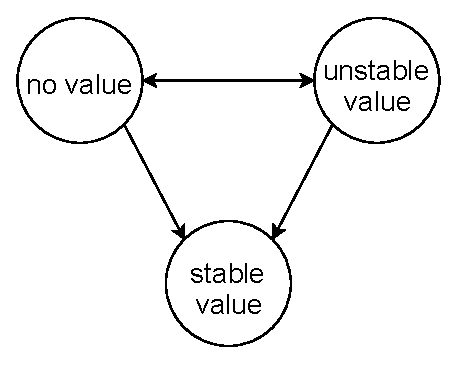
\includegraphics[scale=0.7]{thesis/img/task_value.eps}
\end{center}
\caption{Possible states of a \texttt{TaskValue}}
\label{fig:task_value}
\end{figure}

A Task can be of any type, as long as it provides instances for the type classes in the \texttt{iTask} type class collection. These instances can be automatically derived or explicitly declared. Automatic derivation is available for any first-order type as long as it is not abstract. Basic types have instances already defined in the iTasks library. Explicit declaration allows the user to define custom instances of the \texttt{iTask} class collection if the default derived instance is not suitable. Moreover, it allows instances for extendable, abstract and the function types. 

\section{Interaction}\label{interaction}

The iTasks library provides basic tasks for user interaction. Listing \ref{l_top1} shows the three basic interactive tasks: \texttt{enterInformation}, \texttt{viewInformation} and \texttt{updateInformation}. They create user interface elements to enter, view and update information respectively. As seen in Listing \ref{l_top1}, these basic tasks include a class constraint on the type of the returned \texttt{Task}. This constraint enforces that the type \texttt{m} has an instance of the \texttt{iTask} type class. 

\begin{lstlisting}[caption=iTasks basic interaction functions,captionpos=b,label=l_top1]
enterInformation  :: d [EnterOption m]      -> Task m | iTask m
viewInformation   :: d [ViewOption m] m     -> Task m | iTask m
updateInformation :: d [UpdateOption m m] m -> Task m | iTask m 
\end{lstlisting}


Listing \ref{l_top2} displays examples of how to use the basic interactive tasks. First, a new \ac{adt} called \texttt{Location} is introduced. Next, its instance of \texttt{iTask} is automatically derived. Following, a new example \texttt{Location} is introduced. Finally, new tasks are defined in terms of the basic tasks presented in Listing \ref{l_top1}. 


\begin{lstlisting}[caption=Example of basic iTasks interaction functions,captionpos=b,label=l_top2]
:: Location = { city :: String, state :: String }

derive class iTask Location

location :: Location
location = { city="Omaha", state="Nebraska" }

enterLocation :: Task Location
enterLocation = enterInformation "Enter the location" []

viewLocation :: Task Location
viewLocation = viewInformation "View the location" [] location

updateLocation :: Task Location
updateLocation = updateInformation "Update the location" [] location
\end{lstlisting}

Figure \ref{fig:itasks_display} displays the user interfaces generated for the basic tasks \texttt{enterInformation} (Figure \ref{fig:enter_info}), \texttt{viewInformation} (Figure \ref{fig:view_info}) and \texttt{updateInformation} (Figure \ref{fig:upd_info}).

\begin{figure}[H]
\begin{subfigure}{0.33\textwidth}
\includegraphics[scale=0.7]{thesis/img/enter_location.png}
\caption{Enter information}
\label{fig:enter_info}
\end{subfigure}
\begin{subfigure}{0.33\textwidth}
\includegraphics[scale=0.55]{thesis/img/view_location.png}
\caption{View information}
\label{fig:view_info}
\end{subfigure}
\begin{subfigure}{0.33\textwidth}
\includegraphics[scale=0.7]{thesis/img/update_location.png}
\caption{Update information}
\label{fig:upd_info}
\end{subfigure}
\caption{The visual representation of the basic iTasks interaction functions}
\label{fig:itasks_display}
\end{figure}


\section{Combinators}\label{combinators}

Although the basic tasks introduced in Section \ref{interaction} allow the user to exchange information with the iTasks application, they are quite limited. In order to allow the user to express more complex behavior, task combinators were introduced. Combinators are functions (usually infix operators) that determine how its argument tasks will be combined into a new task. There are only two fundamental composition combinators: sequence and parallel~\cite{top_fl}. All the other combinators in the \texttt{iTask} library are derived from these fundamental combinators. Only the derived combinators will be discussed in this document.

\subsection{Sequential Combinators}

Tasks can be executed in sequence using the \texttt{>>*} combinator, also called the \textit{step} combinator. Its type signature can be seen on Listing \ref{seq_comb}. The step combinator takes a \texttt{Task a} and a list of task continuations as input. A task continuation defines a condition on when to execute another task. It is a predicate that runs on either user actions, task values or thrown exceptions.

\begin{lstlisting}[caption=Sequential combinators,label=seq_comb,captionpos=b]
(>>*) infixl 1 :: (Task a) [TaskCont a (Task b)] -> Task b | iTask a & iTask b

:: TaskCont a b                               
	= OnValue ((TaskValue a) -> Maybe b)         
	| OnAction Action ((TaskValue a) -> Maybe b) 
	| E.e: OnException (e -> b) & iTask e        
	| OnAllExceptions (String -> b)

(>>=) infixl 1 :: (m a) (a -> m b) -> m b   | iTask a & iTask b
(>>|) infixl 1 :: (m a) (m b)     -> m b   | iTask a & iTask b
\end{lstlisting}

The \texttt{>>=} (also called \textit{bind}) is an example of sequential combinator derived from the step combinator. Its first argument is the first task to be executed and its second arguments is a function that takes the first task's value as input and returns a task. The \texttt{>>|} combinator is derived from the bind combinator. It executes two tasks sequentially, but the value of the first task is disregarded. On both \texttt{>>=} and \texttt{>>|}, the second task is executed if either the value of the first task becomes stable, or it is unstable and the user presses a "Continue" button.

\subsection{Parallel Combinators}

Tasks can be executed in parallel using the \textit{parallel} combinator. All the other parallel combinators in the iTasks library are derived from it. Among them, \texttt{-\&\&-} and  \texttt{-||-} are the most commonly used. The first executes two tasks in parallel and returns a tuple containing the result of both argument tasks. The \texttt{-||-} combinator executes two tasks in parallel, but behaves differently from the \texttt{-\&\&-} combinator. The value of the combined task depends on the stability of the argument tasks. If none of the tasks are stable, the combined task yields the last modified non-stable value. If one of the values becomes stable, the combinator yields it, preserving its stability. The type signatures of both combinators can be seen on Listing \ref{par_comb}.

\begin{lstlisting}[caption=Parallel combinators,label=par_comb,captionpos=b]
(-&&-) infixr 4 :: (Task a) (Task b) -> Task (a,b) | iTask a & iTask b
(-||-) infixr 3 :: (Task a) (Task a) -> Task a     | iTask a
\end{lstlisting}


\section{Shared Data Sources}

Albeit task combinators are a powerful tool to 
communicate values among tasks, some applications need to perform ad hoc communication with the external world. \acp{sds} abstract from implementation details on how resources are accessed. A resource can be, for example, a database, a file, the system time or a shared value in memory. 

One approach to create an abstract view on shared data is called a lens~\cite{lenses}. A lens is a bidirectional transformation that provides an interface for reading and writing shared data. Lenses can be extended to allow change notifications: a view is notified when the underlying shared data was modified. Thus, a view always presents updated information. This ability to listen for notifications is called \textit{observing}. Although change notifications are useful, each notification has communication and performance costs. When the shared data is relatively small and seldom updated, no problem arises. Although, if the data is represented by a large data structure that is often updated, broadcasting notifications might impact performance. 

This performance impact could be reduced if lenses were able to filter notifications based on which part of the underlying data was modified. Traditional lenses do not provide a mechanism to encode that information. Parametric lenses are an extension to traditional lenses that enable notification filtering according to a \textit{focus} domain~\cite{parametric}. This focus domain is used to encode notification predicates that tell whether a change on the underlying shared source affects the current view. This way, change notifications can be sent only to the views that are affected by the change, reducing unnecessary notifications.

\acp{sds} are implemented using parametric lenses. As it can be seen from Listing \ref{sds1}, an \texttt{SDS} has three type parameters. The first one is the type of the \textit{focus} domain. The second and third types are the read and write data types respectively. Note that they do not need to be the same type. A \texttt{ReadWriteShared} is an \ac{sds} where the focus domain is of type \texttt{()} (void). A \texttt{Shared} is a \texttt{ReadWriteShared} where read and write types are the same.

% SDS functions
There are four basic functions to operate on \acp{sds}: \textit{get}, \textit{set}, \textit{update} and \textit{watch}. Their type signatures can be seen on Listing \ref{sds1}. The \texttt{get} operation simply fetches the current value of an \ac{sds}. Analogously, the \texttt{set} function sets an \ac{sds}'s value. The \texttt{upd} operation sets the \ac{sds}'s value based on its current value. The \texttt{watch} function continuously reads the value of an \ac{sds}. The \texttt{get}, \texttt{set} and \texttt{update} operations are atomic: during a reading, no other operation is executed.

\begin{lstlisting}[caption=Shared Data Sources definitions,label=sds1,captionpos=b]
:: SDS p r w = ...
:: ReadWriteShared r w :== SDS () r w
:: Shared a :== SDS () a a

get   :: (ReadWriteShared a w)           -> Task a | iTask a
set   :: a (ReadWriteShared r a)         -> Task a | iTask a
upd   :: (r -> w) (ReadWriteShared r w)   -> Task w | iTask r & iTask w
watch :: (ReadWriteShared r w)           -> Task r | iTask r
\end{lstlisting}

\acp{sds} can be composed to create new \acp{sds} using combinators defined in the iTasks library. In addition, interactive tasks equivalent to the ones described in Section \ref{interaction} are defined for the type \texttt{ReadWriteShared}. Their signatures can be seen on Listing \ref{sds2}. Both of these interactive tasks \textit{observe} the \ac{sds}. Therefore, changes on the \texttt{ReadWriteShared} will be automatically displayed.

\begin{lstlisting}[caption=\ac{sds} interactive tasks,label=sds2,captionpos=b]
viewSharedInformation ::   d [ViewOption r]     (ReadWriteShared r w) -> Task r | iTask r 
updateSharedInformation :: d [UpdateOption r w] (ReadWriteShared r w) -> Task r | iTask r & iTask w
\end{lstlisting}

\chapter{The mTask EDSL}
    
\section{IoT and TOP}

\section{Interpreted mTask}

\section{Example}

\chapter{The Application}
    The first step to answer the research question is to choose an application to develop. This chapter presents the criteria used in the selection process and the application chosen: home automation.

\section{Selection Criteria}\label{sec:selec_cri}

The application developed during the research should ideally display the following characteristics:

\paragraph{Suitable} The application should solve a problem that is suitable for mTask. This narrows the choice to \ac{iot} applications that can be developed for one of the platforms that mTask supports.

\paragraph{Non-trivial} The application should not solve a trivial problem --- e.g. a simple hallway  motion-activated light sensor. It should go beyond a purely reactive system. It does not have to solve a novel problem, but its development should be adequately challenging.

\paragraph{Simple} It should be simple enough to be developed during this research. Since we are not aiming for a full-pledged application, some concerns as feature completeness, user experience design and security are not taken into account. Its source code should be neither too complex or big. Ideally, its entire code base would not contain more than 500 lines of code. 

\paragraph{Interesting} It is not enough that the application is suitable and technically good. It should tackle an existing, interesting problem. The application should be well motivated.

\paragraph{Significant} The application should somehow improve the environment it is inserted into. Examples are accelerating an assembly line, saving commute  time, improving one's health or well being or reducing operational cost.

\paragraph{Comprehensible} Its domain and main features should be easily understandable by non-domain experts. Its functionality details and operational features might require specific knowledge, but the application should be easily described on a high level to someone who is not inserted in its domain. Comprehensibility is relevant because it improves the application and therefore the research's reachability. 

\paragraph{Robust} The application should be able to handle errors to some extent. It should at least be able to detect and communicate device disconnection. Ideally, it would automatically migrate tasks from disconnected devices to available devices whenever possible. 

\paragraph{Highly connected} It should support multiple devices simultaneously. These devices should be able to exchange information (e.g. sensor values) when suitable. Ideally, the devices would be connected wirelessly.

\paragraph{Dynamic} The application should not be static. Given that we are exploring the interpreted version of mTask (Section \ref{sec:int_mtask}), we want to exploit its dynamic nature. The application domain should naturally allow dynamicity. Ideally, tasks would be sent to and removed from devices regularly.

\paragraph{Diverse} It should use as many peripherals as possible. Since mTask targets microcontrollers, it is important that a diverse group of sensors and actuators is used. The application should not restrict itself to a couple of peripherals. 

\paragraph{Extensive} The application should use mTask features extensively. Given that it is testing mTask's ability to develop applications, it is important that the application tests as many mTask features as possible. The more features are used by the application, the more confident we are about mTask's abilities.

\section{Home Automation}

Many potential \ac{iot} applications were considered to be developed during research. After a systematic selection process based on the selection criteria described on Section \ref{sec:selec_cri}, a home automation solution was chosen. A detailed analysis of why we chose this domain is presented on Section \ref{sec:app_analysis}.

Home automation might refer to different levels of automation of home tasks. By definition, any tool or machine that automates a home task constitutes a home automation solution. Historically, home automation became popular with the advent of distributed electricity. Daily tasks as dishwashing and drying clothes were automated by appliances that today are common in many households around the world.

In the last decades, home automation gained another meaning with the invention of electronic solutions that control virtually any electronic in a house. Lighting, air conditioners, heaters, entertainment systems and doors are common components controlled by home automation solutions. Frequently, these applications are composed by a central control unit with a user interface (e.g. computer, tablet, smartphone, wall control panel), a communication channel (e.g. Bluetooth, \acs{lan}, Internet, infrared) and devices to be controlled (e.g. lamp, air conditioning unit, doors, TV, appliances).

Automated tasks might be as simple as turning a light on when someone enters the room, controlling the heater based on a target room temperature, locking the main door at a set time and closing the curtains based on the amount of natural light outside. They might also be more elaborated as automatically turning the coffee maker on at 8:00 AM on work days, but only if somebody is home.

\section{Application Description}

The home automation application proposed is called Autohouse. Its goal is to enable and manage the automation of a home (hereafter referred as \textit{smarthome}) using mTask. An Autohouse home is composed by rooms that can be added and removed by its user. Each room contain devices (called \textit{units} in the application) that execute tasks chosen by the user. 

The smarthome management is done in the control panel, a web interface that can be accessed using a web browser. Multiple instances of the control panel can run simultaneously. There, the user has access to the main features of the application:

\begin{itemize}
    \item Manage home: add and remove rooms to the smarthome
    \item Manage room: add and remove units to a room
    \item Send task: send a new task to one of the available units
    \item Stop task: delete a task that is currently running on a unit
    \item Inspect unit: see which tasks are running on a unit
\end{itemize}

\subsection{Architecture}

Autohouse is a centralized solution: a server (ideally located in the home) is the central communication hub for both users and devices. User communication is accomplished via the web control panel, which is hosted in the server. Device communication is accomplished via the mTask library and its communication protocol described in Section \ref{sec:mtask_com_prot}. Figure \ref{fig:autohouse_arch} displays an example architecture of Autohouse deployed on a home with 3 units. 

\begin{figure}[H]
\begin{center}
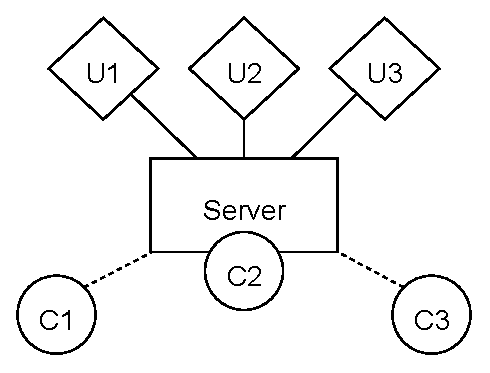
\includegraphics[scale=1.0]{thesis/img/autohouse_arch.eps}
\end{center}
\caption{Autohouse Architecture}
\label{fig:autohouse_arch}
\end{figure}

In Figure \ref{fig:autohouse_arch}, units are represented as diamonds, the server is represented as a rectangle and clients accessing the web control panel are represented as circles. Rooms are just an abstraction layer to ease the use of Autohouse and therefore are not represented in its architecture. Units are microcontrollers equipped with peripherals (sensors, actuators) and an with interface for wireless communication with the server. The server can be any computer with networking capabilities that is supported by Clean and that has enough resources to run the application. A client is a device accessing the control panel using a web browser. Note that the server itself may be a client, since it can access the control panel via a web browser. In addition, if the server is exposed to the Internet, the control panel can be accessed remotely. 

Communication between the server and the units must be persistent (represented by the continuous line between them in Figure \ref{fig:autohouse_arch}). If the communication is interrupted, the server interprets it as a disconnection. Communication between the server and the clients can be transient (represented by the dotted line between them in Figure \ref{fig:autohouse_arch}). Since clients are just managing the application, their connection does not have to be persistent. 

Following one of the criterion introduced in Section \ref{sec:selec_cri}, units should connect to the servers wirelessly. The mTask library supports two types of connections: serial and TCP. Although, which technology is used to establish these connections is irrelevant to the end user. Therefore, Autohouse is technology agnostic in regard to communication between units and the server. Units can, for example, establish a serial connection via Bluetooth or a TCP connection via WiFi. As a consequence, Autohouse does not enforce a wireless connection between the units and the server. The user decides which communication technology is more adequate to their needs.

\subsection{Tasks}

The main purpose of Autohouse is to send automation tasks to units so they can be executed without human supervision. Therefore, the tasks the application supports play a key role in Autohouse. The application should have a list of predefined tasks that are relevant to the house automation domain. The user could pick tasks form this default task list and select a unit to send it to. Initially, there should be no way for the user to add new tasks to the default task list.

The default task list was not previously specified. Given that it was not known in advance which peripherals would be incorporated into Autohouse, creating a task list was not possible. Although, we had an idea of the types of tasks we aimed to implement in Autohouse. Some of these tasks are listed below, from simple reactive tasks to more elaborate ones:

\begin{itemize}
    \item Turn a light on when movement is detected
    \item Turn a light off when the environment is bright enough
    \item Turn the ceiling fan off when there is an object about to hit it
    \item Open or close the curtains based on the brightness inside and outside
    \item Manage the air conditioning unit and the heater based on a target room temperature and on the actual room temperature
    \item Open the windows if the air quality inside is poor and if the outside temperature is acceptable
    \item Turn the coffee maker on at 8:00 AM on work days, but only if somebody is home
\end{itemize}

The tasks that will be implemented into Autohouse will depend on available development time, peripheral support and mTask capability. The last condition is extremely relevant because it directly relates to the research question. If a task could not be implemented due to mTask limitations, we have a hint about how to improve mTask.

\subsection{Devices}\label{sec:autohouse_devices}

Three microcontroller-based platforms are supported by mTask: NodeMCU, STM32 and Arduino. We chose Arduino~\cite{arduino} as the main platform for Autohouse. Arduino is an open-source electronics platform which has single-board microcontrollers specifications and software to support them. We chose Arduino because of its open-source nature, popularity, well-established community, open-source code availability and cost.

The Arduino platform currently has many boards with different specifications and purposes. We chose the Arduino Uno Rev3\footnote{Arduino Uno Rev3. Available at \url{https://store.arduino.cc/arduino-uno-rev3}. Accessed on August 26th 2018}  as the target device because of its popularity, extensibility (using shields\footnote{Arduino Shields. Available at \url{https://www.arduino.cc/en/Main/arduinoShields}. Accessed on August 26th 2018}) and its limited resources. The Arduino Uno is based on the ATmega328P microprocessor, which has only 2 KB of RAM. This memory limitation is a desired characteristic, given that we are testing whether mTask is suitable for microcontrollers, which might include devices with extremely limited resources. The Arduino Uno operates at a frequency of 16 MHz, has 6 analog pins, 14 digital pins, 32 KB of flash memory and a built-in \acs{led}. Its digital and analog pins are often used to interface with peripherals, including sensors and actuators. 

Sensors and actuators are extremely relevant to Autohouse because they allow the application to interface with the real world without human interference. Examples of sensors are temperature, humidity and noise sensors. Examples of actuators are buttons, switches, \acsp{led} and motors.

\subsection{Sensors}

The sensors Autohouse plans to support are relevant to a home environment, both indoors and outdoors. Due to time limitations, not all sensors might be implemented into Autohouse during the research. Ideally, Autohouse would implement the following sensors, from high to low priority: temperature, humidity, light, movement, proximity (ultrasonic), noise, water and air quality sensors. 

\subsection{Actuators}

The actuators Autohouse plans to support are relevant to a home automation application. Due to time limitations, not all actuators might be implemented into Autohouse during the research. Ideally, Autohouse would implement the following actuators, from high to low priority: \acsp{led}, push down buttons, switches, servos and \acsp{lcd}.

\section{Application Analysis}\label{sec:app_analysis}


\chapter{Application Development}
    \section{Development Overview}
\subsection{Application Architecture}
\subsection{Using the Simulator}
\subsection{Device Deployment}
\subsubsection{Devices}
\subsubsection{Peripherals}-
\subsubsection{Communication}

\section{Changes to mTask}
\subsection{Variables}

Since \gls{mTask} is an imperative language, it would benefit from mutable data features. Although there are no \gls{mTask} constructs to represent variables, \acp{sds} might be used as updatable data containers. In such a setting, an \ac{sds} is created for each desired variable. This trick brings updatable data storage to \gls{mTask}, but it prompts two problems. 

First, there is no separation of concerns. Variables and \acp{sds} are by definition, different things. A variable is a \textit{local} updatable data storage in memory. An \ac{sds} is an abstraction layer over any kind of shared data, including data in memory. Using an \ac{sds} locally goes against what a \textit{shared} data source represents. Second, when \acp{sds} are sent to devices, they are not attached to a specific task. Also, on the current version of \gls{mTask}, there is no way to establish whether an \ac{sds} belongs to a given task. As a consequence, \acp{sds} are never deleted from devices. Variables, on the other hand, are always bond to a specific task and could be removed with their correspondent task altogether, saving space in the device's memory. Thus, \gls{mTask} could benefit from a language construct for variables. 

The \texttt{vari} class was created to fill this gap. It contains two functions: \texttt{vari} and \texttt{con}, representing variable and constant data storage respectively. Its definition can be seen in Listing \ref{vari_class}. From a language construct point of view, the \texttt{sds} and \texttt{vari} classes do not differ much. Both classes contain constructs that might be used as updatables and as expressions. But there are two differences between these classes. First, \texttt{vari} contains a construct for constant data: \texttt{con}. Second, \texttt{vari} functions expect a value of type \texttt{t} as its initial value (seen as the first argument of \texttt{In} in Listing \ref{vari_class}). The \texttt{sds} function expects a \texttt{Shared t} instead. The biggest difference between the \texttt{sds} and \texttt{vari} classes regards their behavior on the interpreted view of \gls{mTask}. Variables belong to a task and will live as long as the task lives. \acp{sds} are not bound to a task and will live in the device indefinitely. 


\begin{lstlisting}[caption=The \texttt{vari} class,captionpos=b,label=vari_class]
:: Vari  = Vari
instance isExpr Vari 
instance isUpd Vari 

class vari v where
  vari :: ((v t Vari) -> In t (Main (v c s))) -> (Main (v c s)) 
  con ::  ((v t Expr) -> In t (Main (v c s))) -> (Main (v c s))
\end{lstlisting}

Listing \ref{vari_example} displays an example of variables in \gls{mTask}: the task \texttt{blink}. This task blinks \texttt{LED1} based on the value of variable \texttt{v}. The variable \texttt{v} is created using the \texttt{vari} construct. Its value is updated using the \texttt{=.} infix operator, similarly to \acp{sds}. It can also be used as a boolean expression, as the condition to an \texttt{IF} construct.

\begin{lstlisting}[caption=Example of the usage of variables in mTask,captionpos=b,label=vari_example]
blink :: Main (v () Stmt) | program v
blink = vari \v = False In { main =
	IF (v) (
		ledOn (lit LED1)
	) (
		ledOff (lit LED1)
	) :.
	v =. Not v :. noOp
	}
\end{lstlisting}

The addition of variables to the language required changes on \gls{mTask}'s communication protocol (Section \ref{sec:mtask_com_prot}). When a task is sent to a device, its variables must be sent as well. Therefore, a \texttt{MTTask} message must include the variables used by the given task. Variables are modelled in the \texttt{BCVariable} record. A variable contains a unique (within a task) identifier and its initial value. The \texttt{BCVariable} record and the communication protocol change can be seen in Listing \ref{vari_message}.

\begin{lstlisting}[caption=Change in mTask's communication protocol to accommodate task variables,captionpos=b,label=vari_message]
:: BCVariable = { vid :: Int, vval :: BCValue }

:: MTaskMSGSend
	= MTTask Int MTaskInterval [BCVariable] String
	 ...
\end{lstlisting}

Additionally, the simulator and the client engine were modified to support task variables. When a task is received, its variables are stored. During task execution, variables are fetched and assigned similarly to \acp{sds}. When a task terminates, its variables are removed from the device.

\subsection{Peripherals}

The \gls{mTask} library already supported some of the peripherals \gls{autohouse} planned to use: \acsp{led}, analog and digital pins. Although, new peripherals (e.g. light, temperature and humidity sensors) had to be added to implement some of the proposed automation tasks. Following the natural development process of an \gls{mTask} application, these peripherals were first emulated using the simulator. As more peripherals were implemented, it was clear that the workflow required to add a new peripheral to the system could be improved.

Adding a new peripheral requires changes on different parts of \gls{mTask}. An overview of the necessary changes can be seen below.

\begin{itemize}
    \item A new class that represents the peripheral is added to the language. 
    \item Depending on the peripheral, a new \ac{adt} is created to represent its values (e.g. \texttt{DigitalPin}).
    \item New bytecode instructions are created.
    \item Bytecode encodings are updated to support the new instruction and the possibly new \acs{adt}.
    \item The \texttt{MTaskDeviceSpec} record is updated to include a flag for the new peripheral.
    \item The simulator interpreter is updated to handle new bytecode instructions.
    \item The \gls{cpp} client is updated to handle the new peripheral.
\end{itemize}

The changes on the \gls{cpp} client code depended heavily on the type of peripheral being implemented. Changes on the \gls{clean} code though, were often similar. Previously, peripheral code was scattered around the \gls{mTask} library. Peripheral classes were inside the \texttt{Language} module along with possibly new \acsp{adt}. Instances of the peripheral classes for each \gls{mTask} view were in the respective view's module. The simulator interpreter contained peripheral-specific code. Bytecode encodings for basic types were mixed with encodings for peripheral data types. Overall, adding a new peripheral was particularly cumbersome and extremely error-prone. Finally, there was no separation of concerns whatsoever.

A new modular code architecture for peripherals was introduced to solvethe problems described above. Each peripheral should be defined in its own module. Its type class, \acsp{adt}, bytecode encodings and view instances are defined in that same module. The simulator does not have any peripheral-specific code. Instead of explicit fields for each peripheral, the simulator state record (\texttt{SimState}) contains a list of \texttt{Peripheral}. This new data type is a wrapper around every \gls{mTask} peripheral. Its definition can be seen in Listing \ref{lis:peripheral}. 

\begin{lstlisting}[caption=The \texttt{Peripheral} class,captionpos=b,label=lis:peripheral]
:: Peripheral = E.e: Peripheral e & peripheral e

class peripheral e | iTask e where
	processInst :: BC e -> State SimState (e,Bool)
\end{lstlisting}

The \texttt{peripheral} class was created to enable the removal of peripheral-specific code from the simulator interpreter. Its only function, \texttt{processInst} defines how a peripheral should interpret bytecode instructions (\texttt{BC}). Naturally, a peripheral should only interpret instructions that are relevant to it. The simulator interpreter executes one instruction at a time. If an instruction belongs to \gls{mTask}'s core instruction set (excluding peripheral instructions), the interpreter executes it immediately. If the instruction does not belong to the core instruction set, it is assumed to be a peripheral instruction and it is presented to all simulator peripherals using the \texttt{processInst} function. Once a peripheral responds to an instruction (represented by the \texttt{Bool} on \texttt{processInst} returned value), the interpreter considers the instruction executed and stops looking for a peripheral to execute it. If no peripheral executes the instruction, an error ("instruction unknown") is thrown. 

The addition of new bytecode instructions remains outside of the peripheral module. Although technically it is possible to extend the bytecode data type (\texttt{BC}) in seperate modules, the amount of work necessary to do so outweighed the benefits it could bring. 

The development that followed the changes described above proved that the separation of concerns regarding peripheral code improved \gls{mTask}. Peripherals were added faster, with less code changes and less errors. Additionally, code maintainability increased substantially. Since peripheral code lays mostly in the same module, small changes can be performed faster and safer.

\subsection{Device Requirements}

Some tasks rely on certain peripherals to execute. For example, a task that regulates room temperature relies on a temperature sensor. Despite that, \gls{mTask} does not provide a mechanism to determine whether a task is compatible with a device. The \texttt{Requirements} view was created to bring this feature to \gls{mTask}. Its definition can be seen in Listing \ref{lis:requirements}. \texttt{Requirement} is a type constructor with two phantom type variables: \texttt{a} and \texttt{b}~\cite{phantom}. These type variables are required by the \gls{mTask} type classes. \texttt{Requirement} is a wrapper around the device specification type \texttt{MTaskDeviceSpec}. 

Given a \gls{mTask} construct, this view will return the minimum device specification necessary to support that construct. We can use that information do determine whether a device matches the minimum specification for a task and therefore, if it is compatible with it. The \texttt{match} function does exactly that. Given an \gls{mTask} program and a \texttt{Maybe MTaskDeviceSpec}, it yields whether the device and program are compatible.

\begin{lstlisting}[caption=The \texttt{Requirements} view,captionpos=b,label=lis:requirements]
:: Requirements a b = Req MTaskDeviceSpec

match :: (Main (Requirements a b)) (Maybe MTaskDeviceSpec) -> Bool

instance arith Requirements
instance UserLED Requirements 
\end{lstlisting}

Instances of \gls{mTask} classes (including peripheral classes) are defined for \texttt{Requirement}. Therefore, given a task, an application can filter the available devices based on whether they are compatible with it. The opposite is also possible: given a device, an application can filter tasks based on whether they are compatible with it.

\subsection{Device Disconnection}

By design, \gls{autohouse} should be robust regarding device disconnection (Section \ref{sec:app_analysis}). Ideally, the system would detect a device disconnection and migrate the device's tasks to another suitable device. There were two challenges to tackle in order to implement this feature. 

First, \gls{mTask} does not recognize device disconnection for all of the device types it supports. Simulators never get disconnected. \acs{tcp} devices throw an \gls{iTasks} error when a disconnection is identified. This error is not caught by mTask and propagates upwards. Serial devices kill the application when disconnected. The library used by \gls{mTask} to connect to Serial devices (CleanSerial\footnote{CleanSerial on GitLab. Available at \url{git@gitlab.science.ru.nl:mlubbers/CleanSerial.git}. Accessed on Semtember 8th 2018}) halts execution when a device is disconnected. 

In order to detect device disconnection, \gls{mTask} had to be modified. If the device communication fails, the \texttt{channelSync} task (Section \ref{sec:mtask_devices}) should throw an exception\footnote{An \gls{iTasks} Task yields either a value or an exception. The \gls{iTasks} standard library provides functions to create and handle exceptions.}. \acs{tcp} devices already throw an exception when communication fails and therefore require no change. Although simulators never disconnect from the system, simulating a disconnection would benefit testing. Hence, simulators were modified to support intentional disconnection. CleanSerial was modified to support device disconnection recognition. At this point, \gls{mTask} recognizes device disconnection, but does not communicate it to \gls{autohouse}. 

Ideally, \gls{mTask} would communicate device disconnection through an error handler that would be provided by the application. Thus, the application would decide what task to perform in case of a disconnection. As seen in Section \ref{sec:mtask_devices}, the \gls{mTask} library provides a single function to connect with a device: \texttt{withDevice}. This function is responsible (besides other tasks) to manage the connection to the device. It was modified to accommodate an exception handler. Listing \ref{with_device} displays the type signature of the original \texttt{withDevice} along with its new version, named \texttt{withDevice'} here.

\begin{lstlisting}[caption=Change in mTask to allow device disconnection handler,captionpos=b,label=with_device]
withDevice  :: a (MTaskDevice -> Task b)                    -> Task b | channelSync a

withDevice' :: a (MTaskDevice -> Task b) (String -> Task ()) -> Task b | channelSync a
\end{lstlisting}

Consequently, \gls{mTask} recognizes and provides an exception handler for device disconnection. \gls{autohouse} uses this feature to detect Unit disconnection and thus automatically migrate tasks from the disconnected device to a suitable one.

\subsection{Simulator Improvements}

The simulator (Section \ref{mtask_simulator}) proved to be an essential tool during the development of \gls{autohouse}. Although, it was clear that it could be improved to ease debug and testing of the application. 

Sometimes, the developer might want to debug a task and inspect it closely. The simulator's manual mode is adequate for such usage, but it might be a bit cumbersome to use. Specially with large tasks, stepping over each program instruction becomes a rather tedious and inefficient process. With that in mind, the simulator was extended to support breakpoints on bytecode instructions. Tools to add and to step over breakpoints were added to the simulator \acs{ui}. When executing a task, the simulator goes through its bytecode instructions, checking if there are breakpoints on each instruction before executing it. If an instruction has a breakpoint, execution awaits for user input (by clicking on "step over") to continue. At any point, the user is able to edit breakpoints. 

The ability to simulate peripheral values is crucial for program testing in \gls{mTask}. Tasks often rely on peripheral values and therefore can only be thoroughly tested if peripheral values can be simulated. Although, the simulator did not have such feature. The development of \gls{autohouse} showed how necessary this feature is for \gls{mTask} development. Hence, simulation of peripheral values was incorporated to the simulator. Values can be manually set via the simulator \acs{ui}, similarly to breakpoints. 

\section{Task Migration}



\chapter{Conclusion}
    \section{Discussion}
\section{Future Work}
\section{Conclusion}

The research reported in this documented tested \gls{mTask}'s ability to develop real-life \acs{iot} applications. The research question was tackled by example: the \gls{autohouse} application intended to assess \gls{mTask}'s capabilities. The application is a home automation system that allows users to dynamically manage automation tasks running on devices spread across different rooms. 

Limitations of \gls{mTask} surfaced during the development of \gls{autohouse}. Some limitations were overcome by changing the \gls{mTask} and CleanSerial libraries. Task variables were added to the language. Device disconnection recognition was implemented, allowing the application to automatically migrate tasks when a device is lost. A new view was added to the \ac{edsl} which generates minimum device requirements for a \gls{mTask} task. This view can be used to filter available devices based on whether they support a given task. Six new peripherals were added to the \gls{mTask} language and to the \gls{arduino} client. Peripheral code was restructured, easing the addition of new peripherals, increasing code maintainability and bringing a better separation of concerns between the language core constructs and peripheral constructs. Finally, the simulator for the interpreted \gls{mTask} was modified to support the setting of peripheral values and breakpoints, which improved testing and debugging considerably.

Other limitations could not be overcome during this research. \acsp{sds} are never removed from devices and live there indefinitely. There is a communication loop between devices and server whenever a device publishes an \acs{sds}. The \gls{mTask} library does not communicate neither device connection success nor task acknowledgment. Although these limitations were not overcome, they did not stop the development of \gls{autohouse}. 

The \gls{mTask} \acs{edsl} and library were successfully used to develop a real-life \acs{iot} application: the home automation system \gls{autohouse}. Some of the limitations unearthed during the development process were overcome and some remain. Finally, it is clear what the next steps to improve \gls{mTask} are.

\chapter{Related Work}
    Recent research has been conducted on mTask. A new, task-based version of it has been proposed~\cite{micro}. On this version, the imperative language has been replaced by a functional one. This new version was not used during the research reported in this document because its implementation was not available on time.

The usage of programming languages to interface with microcontrollers has been a subject of research. Firmata\footnote{Firmata Protocol Documentation. Available at \url{https://github.com/firmata/protocol}. Accessed on August 10th 2018.} is a protocol to control microcontrollers. Its messages follow the \acs{midi} message format and model mostly commands on analog and digital input and output pins. There is a client-side implementation for the Arduino\footnote{Firmara Arduino. Available at \url{https://github.com/firmata/arduino}. Accessed on August 10th 2018.} and host-side implementations for many programming languages, including a Haskell implementation to communicate with Arduinos called hArduino\footnote{hArduino. Available at \url{http://leventerkok.github.io/hArduino}. Accessed on August 10th 2018.}. Since Firmata is a protocol and not a programming language, full applications can not be built using Firmata solely. Other tools are built on top of it.

The Haskino library enables Arduino programming using Haskell~\cite{haskino}. The library is available in two different flavors. The first one is based on hArduino (and consequently, on Firmata) and requires the Arduino to maintain a serial connection with the host. On this approach, most of the program evaluation is executed on the host and only I/O commands run on the client. The second approach drops Firmata and uses its own communication protocol. The client is more independent and can execute more elaborate commands, including control flow constructs. In contrast with the first approach, it presents a lower communication overhead. In addition, programs can be written to the Arduino's \acs{eeprom}, allowing standalone execution.

Some research has been made on generating C/C++ code for microcontrollers from high level languages. Ivory is an \ac{edsl} embedded into Haskell that generates safe embedded C code~\cite{ivory1,ivory2}. By design, the generated code is memory safe and free from common errors and undefined behaviors. It uses Haskell's type system (with some \acs{ghc} extensions) to avoid errors like array indexing out of bounds, main loop function with return statements and dangling pointers. Additionally, it prohibits (by design) some standard C features that might generate unsafe code. Ivory was used on the development of the SMACCPilot, a high-assurance autopilot system for quadcopter \ac{uav}.

The \texttt{frp-arduino} library\footnote{\acs{frp} on Arduino. Available at \url{https://github.com/frp-arduino/frp-arduino}. Accessed on August 10th 2018.} implements the \ac{frp} paradigm as an \ac{edsl} embedded in Haskell. Programs in the \ac{edsl} can be compiled to Arduino C code which can be uploaded to Arduino boards. Juniper\footnote{Juniper Programming Language. Available at \url{http://www.juniper-lang.org/index.html}. Accessed on August 11th 2018.} is another \ac{frp} language for the Arduino. It is a standalone programming language that transpiles to Arduino C++.

Additionally, some programming language interpreters were ported to microcontrollers. Espruino\footnote{Espruino. Available at \url{https://www.espruino.com}. Accessed on August 10th 2018.} is a JavaScript interpreter for microcontrollers. It officially supports only proprietary boards but other microcontrollers such as the ESP8266 and the members of the STM32 family are supported by the community. Due to hardware limitations, none of the Arduino boards are supported. Espruino's official website lists many projects that were built using it, including home automation applications. 

Micropython\footnote{Micropytohn. Available at \url{https://micropython.org}. Accessed on August 10th 2018.} is a lean implementation of the Python interpreter and parts of its standard library for microcontrollers. Its main target device is the proprietary \textit{pyboard}. Given that it requires at least 16KB of RAM, it is not compatible with most Arduino boards. It is compatible with microcontrollers of the STM32 family. Many projects (including home automation) were developed using Micropython and \textit{pyboards}. 

Finally, the programming of microcontrollers dynamically (without the need to plug it to a computer) is a well known practice. For example, the ESP8266\footnote{ESP8266 Overview. Available at \url{https://www.espressif.com/en/products/hardware/esp8266ex/overview}. Accessed at August 11th 2018.} Wi-Fi module supports \ac{ota} programming. The Arduino Uno Wi-Fi\footnote{Arduino Store - Arduino Uno Wi-Fi. Available at \url{https://store.arduino.cc/arduino-uno-wifi}. Accessed on August 11th 2018.} is a version of the Arduino Uno board that contains an ESP8266 module and supports \ac{ota} programming natively via the Arduino \acs{ide}. It is important to note that although \ac{ota} enables dynamic programming of microcontrollers, it differs from mTask's dynamicity. On \ac{ota} programming, the device memory is reset when a new program is loaded. On the dynamic version of mTask, the device's memory and the tasks running on it are unaffected.

% ----------------------------

\backmatter{}

% ------- Bibliography -------
\cleardoublepage
\nocite{*}
\phantomsection
\addcontentsline{toc}{chapter}{Bibliography}
\printbibliography[]
% ----------------------------

% -------- Glossaries --------
\cleardoublepage
\printglossaries
% ----------------------------

% --------- Listings ---------
\cleardoublepage
\phantomsection
\addcontentsline{toc}{chapter}{Listings}
\lstlistoflistings
% ----------------------------

\end{document}